\chapter{Vdev, Labels, and Boot Block}\label{chap:vdev}

\section{Virutal Devices}

ZFS storage pools are made up of a collection of virtual devices.
There are two types of virtual devices: physical virtual devices
(sometimes called leaf vdevs)
and logical virtual devices
(sometimes called interior vdevs).
A physical vdev,
is a writeable media block device (a disk, for example).
A logical vdev is a conceptual grouping of physical vdevs.

Vdevs are arranged in a tree with physical vdev existing as leaves of the tree.
All pools have a special logical vdev called the “root” vdev
which roots the tree.
All direct children of the “root” vdev (physical or logical) are called top-level vdevs.
Illustration~\ref{fig:vdev_sample} shows a tree of vdevs
representing a sample pool configuration containing two mirrors.
The first mirror (labeled “M1”) contains two disk,
represented by “vdev A” and “vdev B”.
Likewise, the second mirror “M2” contains two disks represented by “vdev C” and “vdev D”.
Vdevs A, B, C, and D are all physical vdevs.
“M1” and M2” are logical vdevs;
they are also top-level vdevs since they originate from the “root vdev”.

\begin{figure}
  \centering
  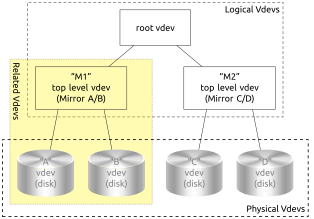
\includegraphics[scale=1]{Figures/zfs_vdev.pdf}
  \caption{Vdev Tree Sample Configuration}
  \label{fig:vdev_sample}
\end{figure}

\section{Vdev Labels}

Each physical vdev within a storage pool contains a 256KB structure called a \emph{vdev label}.
The vdev label contains information
describing this particular physical vdev and all other vdevs
which share a common top-level vdev as an ancestor.
For example,
the vdev label structure contained on vdev “C”, in the previous illustration,
would contain information
describing the following vdevs:
"C", "D", and "M2".
The contents of the vdev label are described in greater detail
in Section~\ref{sec:vdev_detail},
\nameref{sec:vdev_detail}.

The vdev label serves two purposes:
it provides access to a pool's contents
and it is used to verify a pool's integrity and availability.
To ensure that the vdev label is always available and always valid,
redundancy and a staged update model are used.
To provide redundancy,
four copies of the label are written to each physical vdev within the pool.
The four copies are identical within a vdev,
but are not identical across vdevs in the pool.
During label updates,
a two staged transactional approach is used to ensure that
a valid vdev label is always available on disk.
Vdev label redundancy and the transactional update model are described in more detail below.

\subsection{Label Redundancy}

Four copies of the vdev label are written to each physical vdev within a ZFS storage pool.
Aside from the small time frame during label update (described below),
these four labels are identical
and any copy can be used to access and verify the contents of the pool.
When a device is added to the pool,
ZFS places two labels at the front of the device and two labels at the back of the device.
Illustration~\ref{fig:vdev_label} shows the layout of these labels on a device of size N;
L0 and L1 represent the front two labels,
L2 and L3 represent the back two labels.

\begin{figure}[hb]
  \centering
  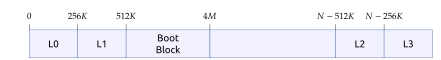
\includegraphics[width=\textwidth]{Figures/zfs_vdev_label.pdf}
  \caption{Vdev Label layout on a block device of size N}
  \label{fig:vdev_label}
\end{figure}

Based on the assumption that
corruption (or accidental disk overwrites) typically occurs in contiguous chunks,
placing the labels in non-contiguous locations (front and back) provides ZFS with a better probability
that some label will remain accessible in the case of media failure or accidental overwrite
(e.g. using the disk as a swap device while it is still part of a ZFS storage pool).

\subsection{Transactional Two Staged Label Update}

The location of the vdev labels are fixed
at the time the device is added to the pool.
Thus,
the vdev label does not have copy-on-write semantics like everything else in ZFS.
Consequently,
when a vdev label is updated,
the contents of the label are overwritten.
Any time on-disk data is overwritten,
there is a potential for error.
To ensure that ZFS always has access to its labels,
a staged approach is used during update.
The first stage of the update writes the even labels (L0 and L2) to disk.
If, at any point in time,
the system comes down or faults during this update,
the odd labels will still be valid.
Once the even labels have made it out to stable storage,
the odd labels (L1 and L3) are updated and written to disk.
This approach has been carefully designed to ensure that
a valid copy of the label remains on disk at all times.

\section{Vdev Technical Details}\label{sec:vdev_detail}
The contents of a vdev label are broken up into four pieces:
8KB of blank space,
8K of boot header information,
112KB of name-value pairs,
and 128KB of 1K sized uberblock structures.
The drawing below shows an expanded view of the L0 label.
A detailed description of each components follows:
blank space
(section \ref{subsec:blankspace}),
boot block header
(section \ref{subsec:bootheader}),
name/value pair list
(section \ref{subsec:nvlist}),
and
uberblock array
(section \ref{subsec:ub}).

\subsection{Blank Space}\label{subsec:blankspace}

ZFS supports both VTOC (Volume Table of Contents) and EFI disk labels
as valid methods of describing disk layout.
\verbfootnote{
Disk labels describe disk partition and slice information.
See \lstinline{fdisk}(\man{1}{m})
and/or \lstinline{format}(\man{1}{m})
for more information on disk partitions and slices.
It should be noted that disk labels are a completely separate entity from vdev labels
and while their naming is similar,
they should not be confused as being similar.
}
While EFI labels are not written as part of a slice
(they have their own reserved space),
VTOC labels must be written to the first 8K of slice 0.
Thus,
to support VTOC labels,
the first 8k of the vdev\_label is left empty to prevent potentially overwriting a VTOC disk label.

\subsection{Boot Block Header}\label{subsec:bootheader}

The boot block header is an 8K structure that is reserved for future use.
The contents of this block will be described in a future appendix of this paper.

\subsection{Name-Value Pair List}\label{subsec:nvlist}

The next 112KB of the label holds a collection of name-value pairs
describing this vdev and all of it's \emph{related vdevs}.
Related vdevs are defined as all vdevs within the subtree rooted at this vdev's top-level vdev.
For example,
the vdev label on device “A”
(seen in Illustration~\ref{fig:vdev_sample}) would contain information
describing the subtree highlighted:
including vdevs “A”, “B”, and “M1” (top-level vdev).

All name-value pairs are stored in \emph{XDR} encoded nvlists.
For more information on XDR encoding or nvlists,
see the \lstinline{libnvpair}(\man{3}{lib})
and \lstinline{nvlist_free}(\man{3}{nvpair}) man pages.
The following name-value pairs (Table~\ref{tbl:nvpair_vdev_label})
are contained within this 112KB portion of the vdev\_label.

\begin{LongTable3Columns}{Name}{Value}{Description}
  {Name-Value Pairs within vdev\_label}{nvpair_vdev_label}
  {@{\extracolsep{\fill}}*{2}{l}p{8.975cm}}
{
  ``version'' & \small{DATA\_TYPE\_UINT64}
  & On disk format version. Current value is ``5000''.\\

  ``name'' & \small{DATA\_TYPE\_STRING}
  & Name of the pool in which this vdev belongs.\\

  ``state'' & \small{DATA\_TYPE\_UINT64}
  & State of this pool. The following table shows all existing pool states.
  The Table~\ref{tbl:pool_states} shows all existing pool states.\\

  ``txg'' & \small{DATA\_TYPE\_UINT64}
  & Transaction group number in which this label was written to disk.\\

  ``pool\_guid'' & \small{DATA\_TYPE\_UINT64}
  & Global unique identifier (guid) for the pool.\\

  ``top\_guid'' & \small{DATA\_TYPE\_UINT64}
  & Global unique identifier for the top-level vdev of this subtree.\\

  ``vdev\_tree'' & \small{DATA\_TYPE\_NVLIST}
  & The vdev\_tree is a nvlist structure which is used recursively
  to describe the hierarchical nature of the vdev tree as seen in illustrations one and four.
  The vdev\_tree recursively describes each “related” vdev witin this vdev's subtree.\\
}
\end{LongTable3Columns}

\begin{LongTable2Columns}{State}{Value}{Pool States}{pool_states}{lr}
{
  POOL\_STATE\_ACTIVE & 0\\
  POOL\_STATE\_EXPORTED & 1\\
  POOL\_STATE\_DESTROYED & 2\\
}
\end{LongTable2Columns}

Each vdev\_tree nvlist contains the elements as described in the Table~\ref{tbl:vdevtree_nvlist_entries}.
Note that not all nvlist elements are applicable to all vdevs types.
Therefore,
a vdev\_tree nvlist may contain only a subset of the elements described below.
The illustration below shows
what the ``vdev\_tree'' entry might look
like for ``vdev A'' as shown in Illustration~\ref{fig:vdev_label}
earlier in this document.

\begin{figure}[hb]
 \centering
  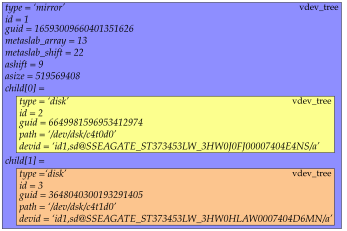
\includegraphics[width=\textwidth]{Figures/zfs_vdev_tree.pdf}
  \caption{Vdev Tree Nvlist Entries}
  \label{fig:vdev_tree} 
\end{figure}

\setlength\LTleft{-1cm}
\setlength\LTright{-1cm}
\begin{LongTable3Columns}{Name}{Value}{Description}
  {Vdev Tree NV List Entries}{vdevtree_nvlist_entries}
  {@{\extracolsep{\fill}}*{2}{l}p{6.8cm}}
{
  ``type'' & \small{DATA\_TYPE\_UINT64}
  & The id is the index of this vdev in its parent's children array.\\

  ``guid'' & \small{DATA\_TYPE\_UINT64}
  & Global Unique Identifier for this vdev\_tree element.\\

  ``path'' & \small{DATA\_TYPE\_STRING}
  & Device path. Only used for leaf vdevs.\\

  ``devid'' & \small{DATA\_TYPE\_STRING}
  & Device ID for this vdev\_tree element. Only used for vdevs of type disk.\\

  ``metaslab\_array'' & \small{DATA\_TYPE\_UINT64}
  & Object number of an object containing an array of object numbers.
  Each element of this array (ma[i]) is, in turn,
  an object number of a space map for metaslab `i'.\\

  ``metaslab\_shift'' & \small{DATA\_TYPE\_UINT64}
  & Log base 2 of the metaslab size.\\

  ``ashift'' & \small{DATA\_TYPE\_UINT64}
  & Log base 2 of the minimum allocatable unit for this top level vdev.
  This is currently 10 for a RAIDz configuration, 9 otherwise.\\

  ``asize'' & \small{DATA\_TYPE\_UINT64}
  & Amount of space that can be allocated from this top level vdev.\\

  ``children'' & \small{DATA\_TYPE\_NVLIST\_ARRAY}
  & Array of vdev\_tree nvlists for each child of this vdev\_tree element.\\
}
\end{LongTable3Columns}
\setlength\LTleft{0pt}
\setlength\LTright{0pt}

\subsection{The Uberblock}\label{subsec:ub}

Immediately following the nvpair lists in the vdev label is an array of \emph{uberblocks}.
\begin{figure}[ht!]
  \centering
  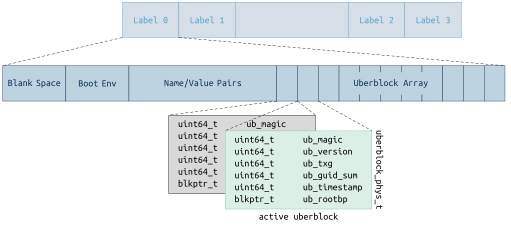
\includegraphics[width=\textwidth]{Figures/zfs_ub_expanded.pdf}
  \caption{Uberblock array showing uberblock contents}
  \label{fig:ub_expanded}
\end{figure}

The uberblock is the portion of the label
containing information necessary to access the contents of the pool.
\verbfootnote{
  The uberblock is similar to the superblock in UFS.
}
Only one uberblock in the pool is active at any point in time.
The uberblock with the highest transaction group number and valid SHA-256 checksum
is the active uberblock.

To ensure constant access to the active uberblock,
the active uberblock is never overwritten.
Instead, all updates to an uberblock are done
by writing a modified uberblock to another element of the uberblock array.
Upon writing the new uberblock,
the transaction group number and timestamps are incremented
thereby making it the new active uberblock in a single atomic action.
Uberblocks are written in a round robin fashion across the various vdevs with the pool.
The Illustration~\ref{fig:ub_expanded}
has an expanded view of two uberblocks within an uberblock array.

\subsubsection{Uberblock Technical Details}

The uberblock is stored in the machine's native endian format and has the following contents:

\begin{description}
\item[ub\_magic]
  The uberblock magic number is a 64 bit integer
  used to identify a device as containing ZFS data.
  The value of the ub\_magic is \verb|0x00bab10c| (oo-ba-block).
  The Table~\ref{tbl:endianess_ub} shows the ub\_magic number as seen on disk.
  \begin{table}[hb]
    \caption{Uberblock values per machine endian type}
    \label{tbl:endianess_ub}
    \centering
    \begin{tabular}{lr}
      \toprule
      \textbf{Machine Endianess} &     \textbf{Uberblock Value}\\
      \midrule
      Big Endian &                     \verb|0x00bab10c|\\
      Little Endian &                  \verb|0x0cb1ba00|\\
      \bottomrule
    \end{tabular}
  \end{table}
  
\item[ub\_version]
  The version field is used to identify the on-disk format in which this data is laid out.
  The current on-disk format version number is ``5000''.
  This field contains the same value
  as the “version” element of the name/value pairs described in Section~\ref{subsec:nvlist}. 

\item[ub\_txg]
  All writes in ZFS are done in transaction groups.
  Each group has an associated transaction group number.
  The ub\_txg value reflects the transaction group in which
  this uberblock was written.
  The ub\_txg number must be greater than or equal to the ``txg'' number
  stored in the nvlist for this label to be valid.

\item[ub\_guid\_sum]
  The ub\_guid\_sum is used to verify the availability of vdevs within a pool.
  When a pool is opened,
  ZFS traverses all leaf vdevs within the pool
  and totals a running sum of all the GUIDs
  (a vdev's guid is stored in the guid nvpair entry, see Section~\ref{subsec:nvlist}) it encounters.
  This computed sum is checked against the ub\_guid\_sum
  to verify the availability of all vdevs within this pool.

\item[ub\_timestamp]
  Coordinated Universal Time (UTC) when
  this uberblock wasf written in seconds since January 1st 1970 (GMT).

\item[ub\_rootbp]
  The ub\_rootbp is a \verb|blkptr| structure containing the location of the MOS.
  Both the MOS and blkptr structures are described in later chapters of this document:
  Chapters~\ref{chap:dsl} and \ref{chap:blkptr} respectively.
\end{description}

\section{Bool Block}

Immediately following the L0 and L1 labels is a 3.5MB chunk reserved for future use
(see Illustration~\ref{fig:vdev_label}).
The contents of this block will be described in a future appendix of this paper.
